\documentclass[a4paper,11pt]{ltjsarticle}

% --- パッケージの読み込み ---
\usepackage{amsmath, amssymb, amsthm, mathrsfs}
\usepackage{luatexja}
\usepackage{tikz}
\usetikzlibrary{cd, shapes, backgrounds, positioning, calc, arrows.meta, fit, patterns, decorations.pathreplacing}
\usepackage{hyperref}
\usepackage{xcolor}
\usepackage{listings}
\usepackage{tcolorbox}
\usepackage{booktabs}
\usepackage{multicol}

% --- ハイパーリンク設定 ---
\hypersetup{
    colorlinks=true,
    linkcolor=blue!70!black,
    citecolor=blue!70!black,
    urlcolor=blue!70!black
}

% --- 定理環境の定義 ---
\theoremstyle{definition}
\newtheorem{definition}{定義}[section]
\newtheorem{theorem}[definition]{定理}
\newtheorem{lemma}[definition]{補題}
\newtheorem{axiom}[definition]{公理}
\newtheorem{remark}[definition]{注釈}

% --- マクロ定義 ---
\newcommand{\N}{\mathbb{N}}
\newcommand{\R}{\mathbb{R}}
\newcommand{\OmegaSpace}{\Omega}
\newcommand{\F}{\mathcal{F}}
\newcommand{\Prob}{\mathbb{P}}
\newcommand{\Expect}{\mathbb{E}}
\newcommand{\CondExp}[2]{\Expect[#1 \mid #2]}
\newcommand{\Tau}{\tau}
\newcommand{\SigmaAlg}{\Sigma}

% --- タイトル情報 ---
\title{\textbf{構造塔による確率論の再構築} \\ \large --- 幻の初期フィルトレーションからDoob分解まで ---}
\author{
    Lean Code Generation: \textbf{CODEX (OpenAI)} \\
    TeX Explanation \& Typesetting: \textbf{Gemini (Google)}
}
\date{\today}

\begin{document}

\maketitle

\begin{abstract}
本稿では、Lean 4ファイル群に基づき、確率論を「構造塔 (Structure Tower)」の枠組みで形式化するプロセスを解説する。
まず、\texttt{Probability.md} における素朴なフィルトレーション定義（幻の初期版）から出発し、それが \texttt{Probability\_Extended.md} で構造塔として洗練される過程を追う。
その後、抽象的な条件付き期待値を導入し、マルチンゲール、任意停止定理、Doob分解、そして停止時間の代数構造へと至る一連の理論展開を数学的に記述する。
\end{abstract}

\tableofcontents
\newpage

% =========================================================================
% Section 1: Probability & Extended - 基礎
% =========================================================================
\section{フィルトレーションの進化：集合から構造塔へ}
\label{sec:foundations}
\textit{Based on: \texttt{Probability.md}, \texttt{Probability\_Extended.md}}

確率論の舞台となる「情報の流れ」をどのように定義するか。ここには2つの段階がある。

\subsection{幻の初期版：素朴な離散フィルトレーション}
\texttt{Probability.md} では、フィルトレーションは単なる「時刻とともに増大する事象の族」として定義される。

\begin{definition}[DiscreteFiltration]
標本空間 $\OmegaSpace$ 上の離散フィルトレーション $F$ とは、自然数 $n \in \N$ で添字付けられた集合族 $(\Sigma_n)_{n \in \N}$ であり、以下を満たすものである。
\begin{enumerate}
    \item $\Sigma_n \subseteq \text{Set}(\OmegaSpace)$
    \item \textbf{単調性}: $n \le m \implies \Sigma_n \subseteq \Sigma_m$
    \item \textbf{被覆性}: 任意の $E \subseteq \OmegaSpace$ に対し、ある $n$ で $E \in \Sigma_n$ となる（※これはかなり強い仮定だが、有限的な設定では自然である）。
\end{enumerate}
\end{definition}

ここでの停止時間 $\Tau$ は、各時刻 $n$ において事象 $\{\omega \mid \Tau(\omega) \le n\}$ が $\Sigma_n$ に含まれるような写像として定義される。

\subsection{拡張版：構造塔としての再解釈}
\texttt{Probability\_Extended.md} において、このフィルトレーションは \texttt{StructureTowerWithMin}（最小層を持つ構造塔）へと昇華される。

\begin{theorem}[フィルトレーションの構造塔化]
フィルトレーション $F$ は、以下の対応により構造塔と見なせる。
\begin{itemize}
    \item \textbf{Carrier}: $\text{Set}(\OmegaSpace)$ （事象全体）
    \item \textbf{Layer $n$}: $\Sigma_n$ （時刻 $n$ での可測事象）
    \item \textbf{minLayer}: 事象 $E$ が初めて可測になる時刻
\end{itemize}
\end{theorem}

これにより、確率論的な「適合性 (Adaptedness)」や「停止 (Stopping)」が、順序構造上の普遍的な操作として扱えるようになる。

\begin{figure}[h]
\centering
\begin{tikzpicture}[scale=1.5]
    % Layers
    \draw[fill=blue!10, dashed] (-2,0) rectangle (4,2.5);
    \node at (3.5, 2.3) {$\OmegaSpace$};
    
    \draw[fill=white] (0,0.5) ellipse (1.5 and 0.8);
    \node at (0, 0.5) {$\Sigma_0$};
    
    \draw[fill=white, fill opacity=0] (0.5,0.5) ellipse (2.5 and 1.5);
    \node at (2.5, 1.0) {$\Sigma_1$};
    
    \node at (3.5, 0.2) {$\Sigma_0 \subseteq \Sigma_1 \subseteq \dots$};
    
    % Stopping Time Cut
    \draw[red, thick] (-1.5, 2) -- (0, 0.5) -- (2, 1.5) -- (3.5, 2);
    \node[red, above] at (0, 1.8) {停止時間 $\Tau$ による「切断面」};
\end{tikzpicture}
\caption{フィルトレーションの包含関係と停止時間のイメージ}
\end{figure}

% =========================================================================
% Section 2: Martingale Guide
% =========================================================================
\section{マルチンゲールの抽象定義}
\label{sec:martingale}
\textit{Based on: \texttt{Level2\_1\_Martingale\_Guide.md}}

測度論的な積分を直接扱うのではなく、公理的な「条件付き期待値作用素」を用いてマルチンゲールを定義する。

\subsection{条件付き期待値の公理}
構造体 \texttt{ConditionalExpectationStructure} は、以下の性質を持つ作用素 $C_n: (\OmegaSpace \to \R) \to (\OmegaSpace \to \R)$ を提供する。
\[ \text{Tower Property}: \quad m \le n \implies C_m(C_n(X)) = C_m(X) \]
これは $\CondExp{\CondExp{X}{\F_n}}{\F_m} = \CondExp{X}{\F_m}$ の抽象化である。

\subsection{マルチンゲール・サブ/スーパーマルチンゲール}
確率過程 $X = (X_n)$ に対し、以下のように定義する。
\begin{itemize}
    \item \textbf{マルチンゲール}: $m \le n \implies C_m(X_n) = X_m$
    \item \textbf{サブマルチンゲール}: $m \le n \implies X_m \le C_m(X_n)$
    \item \textbf{スーパーマルチンゲール}: $m \le n \implies C_m(X_n) \le X_m$
\end{itemize}
ここで「適合性」は、事象 $\{X_n \le r\}$ が $\Sigma_n$ に属することとして定義される。

% =========================================================================
% Section 3: Optional Stopping
% =========================================================================
\section{任意停止定理 (Optional Stopping)}
\label{sec:ost}
\textit{Based on: \texttt{Level2\_2\_OptionalStopping.md}}

構造塔の枠組みにおける停止過程 $X^\Tau$ の定義と、有界停止時間に対する定理。

\subsection{停止過程}
停止時間 $\Tau$ に対する停止過程 $X^\Tau$ は以下で定義される。
\[ X^\Tau_n(\omega) := X_{\min(n, \Tau(\omega))}(\omega) \]
これは、時刻 $\Tau(\omega)$ 以降、値が凍結されることを意味する。

\subsection{有界OST (代数的証明)}
もし $\Tau$ が有界（$\forall \omega, \Tau(\omega) \le N$）であり、期待値汎関数 $E$ が $E[C_0(Y)] = E[Y]$ を満たすならば、マルチンゲール $X$ に対して以下が成り立つ。
\[ E[X_\Tau] = E[X_0] \]
証明は、タワー性 $C_0(X^\Tau_N) = X^\Tau_0 = X_0$ を用いた純粋な代数計算として完結する。

% =========================================================================
% Section 4: Doob Decomposition
% =========================================================================
\section{Doob分解：構造の分離}
\label{sec:doob}
\textit{Based on: \texttt{Level2\_3\_DoobDecomposition*.md}}

確率過程を「公平な賭け（マルチンゲール）」と「予測可能な傾向（ドリフト）」に分解する。

\subsection{予測可能過程 (Predictable Process)}
過程 $A$ が予測可能であるとは、直感的には $A_n$ が $\F_{n-1}$ 可測であることを指すが、本形式化では簡単のため「$A_0$ が定数である」ことなどを基本要請として扱う（詳細な可測性は公理または構成に委ねられる）。

\subsection{分解定理 (存在と一意性)}
任意の適合過程 $X$ は、マルチンゲール $M$ と予測可能過程 $A$ の和として一意に分解できる。
\[ X_n = M_n + A_n, \quad A_0 = 0 \]
ここで $A_n$ は以下のように構成的（あるいは帰納的）に定まる。
\[ A_{n+1} - A_n = \CondExp{X_{n+1} - X_n}{\F_n} \]
Leanファイルでは、この分解の存在と一意性を公理（\texttt{axiom}）として導入し、その操作的性質（線形性など）を導出している。

\begin{figure}[h]
\centering
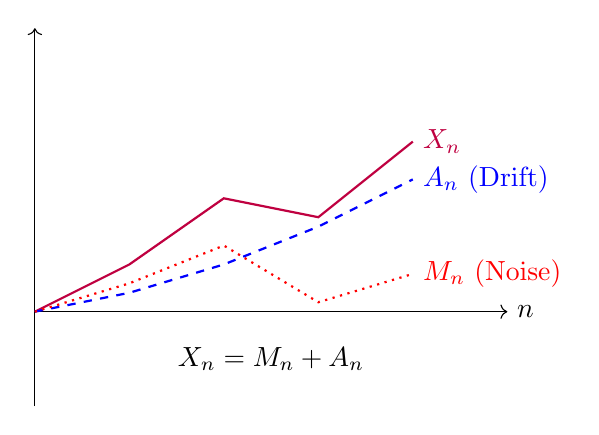
\begin{tikzpicture}[scale=1.2]
    \draw[->] (0,0) -- (5,0) node[right] {$n$};
    \draw[->] (0,-1) -- (0,3);
    
    % X (Total)
    \draw[thick, purple] (0,0) -- (1,0.5) -- (2,1.2) -- (3,1.0) -- (4,1.8) node[right] {$X_n$};
    
    % A (Predictable Drift)
    \draw[thick, blue, dashed] (0,0) -- (1,0.2) -- (2,0.5) -- (3,0.9) -- (4,1.4) node[right] {$A_n$ (Drift)};
    
    % M (Martingale Fluctuation)
    \draw[thick, red, dotted] (0,0) -- (1,0.3) -- (2,0.7) -- (3,0.1) -- (4,0.4) node[right] {$M_n$ (Noise)};
    
    \node at (2.5, -0.5) {$X_n = M_n + A_n$};
\end{tikzpicture}
\caption{Doob分解のイメージ。観測値 $X$ は、予測可能な傾向 $A$ とランダムな変動 $M$ に分解される。}
\end{figure}

% =========================================================================
% Section 5: Stopping Time Algebra
% =========================================================================
\section{停止時間の代数構造}
\label{sec:algebra}
\textit{Based on: \texttt{Level2\_5\_StoppingTimeAlgebra.md}}

停止時間の全体は、順序構造に関して束（Lattice）をなす。

\subsection{点ごとの順序と演算}
停止時間 $\sigma, \tau$ に対し、順序 $\sigma \le \tau$ を $\forall \omega, \sigma(\omega) \le \tau(\omega)$ で定義する。
このとき、以下もまた停止時間となる。
\begin{itemize}
    \item \textbf{最小値}: $(\sigma \land \tau)(\omega) = \min(\sigma(\omega), \tau(\omega))$
    \item \textbf{最大値}: $(\sigma \lor \tau)(\omega) = \max(\sigma(\omega), \tau(\omega))$
    \item \textbf{和}: $(\sigma + \tau)(\omega) = \sigma(\omega) + \tau(\omega)$
\end{itemize}

\subsection{構造塔による解釈}
構造塔の視点では、これらの演算は層の集合演算に対応する。
\[ \{\sigma \land \tau \le n\} = \{\sigma \le n\} \cup \{\tau \le n\} \]
これは「どちらかが $n$ までに起これば、最小値も $n$ までに起きている」ことを意味する。

\section{結論}
一連のLeanファイルは、確率論を「解析」から「代数・順序構造」へと翻訳する試みである。
\begin{enumerate}
    \item \textbf{フィルトレーション}は構造塔として形式化され、情報の増大を表現する。
    \item \textbf{マルチンゲール}は構造塔上の不変量として定義される。
    \item \textbf{Doob分解}は、過程を構造的要素（不変量＋予測可能量）に分解する定理である。
\end{enumerate}
このアプローチにより、確率論の定理が、より抽象的かつ普遍的な「構造の性質」として理解できるようになる。

\end{document}